\documentclass[a4paper, 10pt]{article}

\usepackage{cite}
\usepackage{color}
	\definecolor{gray}{rgb}{0.5,0.5,0.5}
\usepackage{datetime}
\usepackage{fancyvrb}
\usepackage{graphicx}
\graphicspath{{images/}}
\DeclareGraphicsExtensions{.pdf,.png}
%\usepackage{hyperref}
\usepackage{latexsym}
\usepackage{listings}
	\lstset{
		frame=single,
		numbers=left,
		numberstyle=\small\color{gray},
		tabsize=4,
		morekeywords={and, boolean, do, else, false, for, if, integer, mod, true, until, wait, while},
	}
\usepackage{multirow}
\usepackage{setspace}
\usepackage{url}

\def \todo{\textbf{\textcolor{yellow}{TODO}}}
\def \citationneeded{\textbf{\textcolor{yellow}{CITATION NEEDED}}}
\def \listingrule{\rule{12.1cm}{0.4pt}}

\title{Development and Analysis of Barrier Protocols}
\author{Ronny Brendel\\Tutors: Sascha Kl\"uppelholz \& Marcus V\"olp}

\begin{document}
%%%%%%%%%%%%%%%%%%%%%%%%%%%%%%%%%%%%%%%%%%%%%%%%%%%%%%%%%%%%%%%%%%%%%%%%%%%%%%%
\pagenumbering{gobble}

\begin{titlepage}

\begin{center}
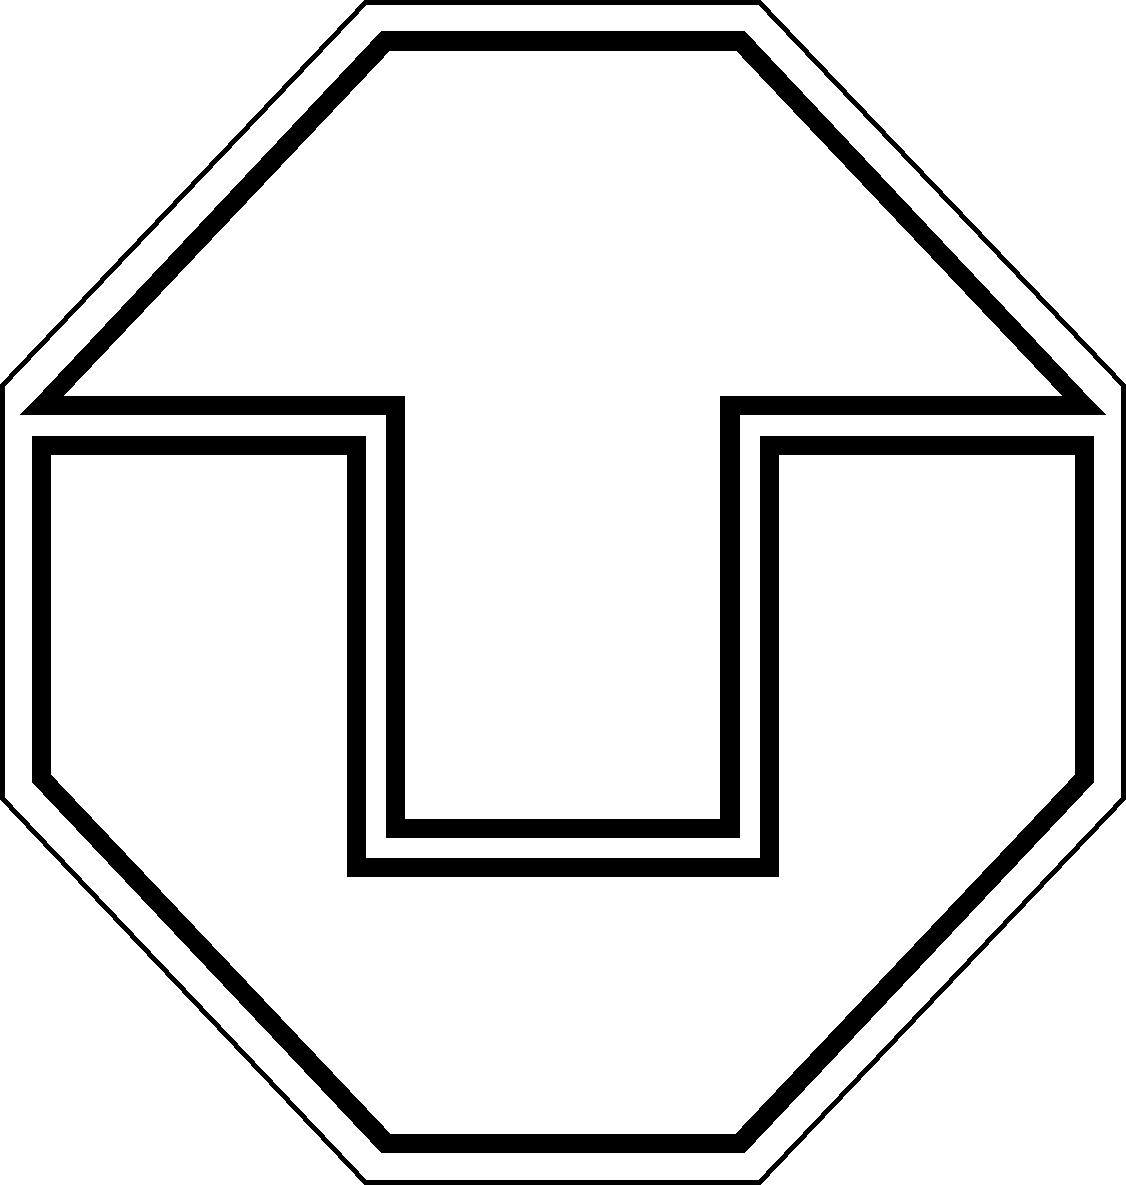
\includegraphics[width=3cm]{tu-logo}~\\[1cm]
\textsc{\LARGE Dresden University of Technology}\\[0.5cm]
\textsc{\Large Faculty of Computer Science}\\[0.2cm]
\textsc{\large Institute of Theoretical Computer Science}\\[0.2cm]
\textsc{\large Chair for Algebraic and Logical Foundations of Computer Science}\\[3cm]
\Huge Study's Thesis \\[1cm]
\huge Development and Analysis of Barrier Protocols\\[3cm]
\end{center}

\begin{flushleft} \large
	Author: Ronny Brendel \\
	Responsible university professor: Christel Baier \\
	Supervisors: Sascha Kl\"uppelholz \& Marcus V\"olp
\end{flushleft}

\vfill
\begin{flushright}
	\large October 2013
\end{flushright}

\end{titlepage}

\pagebreak
\newpage \thispagestyle{empty} \mbox{}
\pagebreak

%%%%%%%%%%%%%%%%%%%%%%%%%%%%%%%%%%%%%%%%%%%%%%%%%%%%%%%%%%%%%%%%%%%%%%%%%%%%%%%
\section*{Aufgabenstellung}

\pagebreak
\newpage \thispagestyle{empty} \mbox{}
\pagebreak

%%%%%%%%%%%%%%%%%%%%%%%%%%%%%%%%%%%%%%%%%%%%%%%%%%%%%%%%%%%%%%%%%%%%%%%%%%%%%%%
%\section*{Selbstst\"andigkeitserkl\"arung}
%Ich erkl\"are hiermit, dass ich die vorliegende Arbeit selbst\"andig und ohne Benutzung anderer als der angegebenen Hilfsmittel angefertigt habe. Die aus fremden Quellen w\"ortlich oder sinngem\"a\ss ~\"ubernommenen Gedanken sind als solche kenntlich gemacht. Ich erkl\"are ferner, dass ich die vorliegende Arbeit an keiner anderen Stelle als Pr\"ufungsarbeit eingereicht habe oder einreichen werde.

\section*{Statement of academic integrity}
I hereby declare that I prepared this thesis independently and without use of tools other than specified. Foreign thoughts, taken literally or in spirit, are marked as such. I also declare that I have not filed the present work at any other location or will submit it.

\pagebreak
\newpage \thispagestyle{empty} \mbox{}
\pagebreak

%%%%%%%%%%%%%%%%%%%%%%%%%%%%%%%%%%%%%%%%%%%%%%%%%%%%%%%%%%%%%%%%%%%%%%%%%%%%%%%
\renewcommand{\contentsname}{Table of contents}
\tableofcontents

\pagebreak
\newpage \thispagestyle{empty} \mbox{}
\pagebreak

%%%%%%%%%%%%%%%%%%%%%%%%%%%%%%%%%%%%%%%%%%%%%%%%%%%%%%%%%%%%%%%%%%%%%%%%%%%%%%%
\pagenumbering{arabic}
\section{Don't forget}
\begin{itemize}
	\item try all algorithms with processor counts $\neq 2^i$ especially dissemination
	\item explain use of 'thread' and 'process'
	\item explain the basic figure style somewhere
		\begin{itemize}
			\item C-esque pseudo-code
			\item threadCount/processCount
			\item threadIndex/processIndex
			\item the code in the figures is executed on each thread. Each thread has an identifier between 0 and threadCount-1
			\item \& bit-wise \texttt{AND}
			\item $|$ bit-wise \texttt{OR}
			\item $\sim$ bit-wise \texttt{NOT}
			\item \texttt{x[$*$] := y} is short for assigning y to each element in x
			\item ?more?
		\end{itemize}
	\item maybe, explain model checking slang somewhere. Probabilistic ltl, pctl formulas. See bai13\cite{bai13} subsection preliminaries.
	\item mention somewhere that we assume atomic read and write at 32/64 bit a piece
\end{itemize}
%%%%%%%%%%%%%%%%%%%%%%%%%%%%%%%%%%%%%%%%%%%%%%%%%%%%%%%%%%%%%%%%%%%%%%%%%%%%%%%

\section{Introduction}
\begin{itemize}
	\item what is a barrier: synchronization mechanism where ...
	\item usage example for barriers. Use example from complex lab?
	\item explain that barriers are very common in parallel programming. OpenMP's\cite{openmp} implicit barriers. MPI barriers (Rolf Rabenseifner\cite{rab00}). Relate to normal send/recv, because absolute numbers without relation are not helpful.
		\begin{itemize}
			\item HLRS, year 2000
			\item many calls,
			\item 5.3\% of all time spent inside MPI calls, 0.7\% of all CPU time, estimated 1.6\% of the barrier execution time is actual synchronization, 100\% minus 1.6\% is waiting for other processes to arrive, because of unbalanced computation, average 1852 micro seconds per call. (Figure~13 in paper)
			\item e.g. receive 12.9\% of all time spent inside MPI calls, 1.8\% of all cpu time, 33\% of the recv executation time is actual latency plus transfer time, 100\% minus 33\% is waiting for other processes to arrive, because of unbalanced comoputation, average 498 micro seconds per call.
		\end{itemize}
	\item motivation for researching barriers: Apply ideas of pW/CS\cite{pwcs} to other synchronization primitives, e.g. barriers.
	\item summarize pW/CS
		\begin{itemize}
			\item usually concurrent programs work in a deterministic fashion. That is the order and partners of remote synchronization (locally, programs are obviously mostly deterministic) are predetermined. The algorithm is executed in a very controlled fashion. Same holds for synchronization primitives themselves. Faulty behavior is avoided at great cost.
			\item don't avoid inconsistency at all cost. Make errors detectable, or ignorable.
			\item use the inherent randomness\cite{mcg09}, induced by caching, scheduling, randomness (ECC, flash access e.g.) at hardware level (jitter), or short: complexity of today's computer systems, in order to view concurrent accesses as really random. Thus we are able to apply probabilistic algorithms and analyse these algorithms using tools of probability theory.
			\item design algorithms that have sufficiently high probability of success and tolerate faulty behaviour.
			\item build them so that on average, or in their intended use case, they perform better than their deterministic counterparts, where better might e.g. be faster, more energy efficient, resource preserving.
			\item data on the success is still rare, but it seems to be promising approach
		\end{itemize}
	\item how do we gather data on these algorithms to build confidence that they work properly, i.e. satisfy certain properties?
	\item Testing/Sampling this is hard or not super-useful:
		\begin{itemize}
			\item where to put this citation bai13~\cite{bai13}?
			\item testing is usually deterministic. If so, certain states in the protocol are impossible to reach because of the randomness inherent in computers (add a short example? A special very case of a low level lock being contented?)
			\item Assuming you have randomized tests, the probability to reach certain states in the protocol is so low that they are not revealed.
			\item modelling does not have these draw backs. Of course it does have others.
			\item we can gain better quantitative insights into protocols through modeling than with testing.
			\item therefore we apply model checking techniques to investigate barriers
		\end{itemize}
	\item what we attempt in this report: (overarching thesis / continuous thread)
		\begin{itemize}
			\item today's barriers can be improved upon. New barriers.
			\item softening the need for determinism in order to gain an advantage is a viable approach to take a stab at today's low level synchronization primitives, or in general. New barriers.
			\item probabilistic model checking is powerful and apt for investigating barriers. Compare the barriers using this.
		\end{itemize}
	\item briefly explain the report structure
		\begin{itemize}
			\item means to implement barriers
			\item currently used barriers
			\item new barriers
			\item analysis and comparison of one old for shared memory and one old for distributed memory against the new barriers
			\item idea to split barriers into orthogonal parts and think about them separately
			\item conclusion \& future work
		\end{itemize}
\end{itemize}


%%%%%%%%%%%%%%%%%%%%%%%%%%%%%%%%%%%%%%%%%%%%%%%%%%%%%%%%%%%%%%%%%%%%%%%%%%%%%%%
\section{Means to implement barrier protocols}
\begin{itemize}
	\item \todo still feels like there should be some kind of wrap up or continuous thread :(
	\item evaluate what tools / APIs we have at our disposal to realize barrier protocols
	\item distinction between shared and distribute memory:
	\item shared memory: all threads share one global memory. They are thus able to communicate by just writing to and reading from memory.
	\item distributed memory: each process has its own private memory. Computation can only be done on private memory. Communication is explicitly done via an interconnect.
	\item programming these two memory architectures is very different, thus subsequently we will differentiate these two worlds.
\end{itemize}

%%%%%%%%%%%%%%%%%%%%%%%%%%%%%%%%%%%%%%%
\subsection{Shared memory}
\begin{itemize}
	\item normal load/store.
	\item atomic ops. An atomic operation is done in one instant without being interrupted by other memory accesses. E.g. add-fetch, compare-swap (is as old as 1970. No citations found. And perhaps not necessary). Never faster than normal read/write. (don't elaborate too much since we want a very high level view of the tools at our disposal)
	\item weaken consistency model. Consistency models describe restrictions on the order of visibility of memory accesses between multiple threads. In a thread, locally, the order is always the one specified by the program -- sequential. The default on x86 and most restrictive consistency model is sequential consistency. It is defined as follows:
		\begin{quote}
			The result of any execution is the same as if the operations of all the processors were executed in some sequential order, and the operations of each individual processor appear in this sequence in the order specified by its program. -- Lamport~\cite{sequentialconsistency}
		\end{quote}
		The most prominent weaker memory consistency model is release consistency~\cite{gha90}. Memory accesses appear unordered except so called \emph{release} and \emph{acquire} operations. No memory access that has been issued after an acquire operation is permitted to finish before this acquire operation. No memory access is allowed to finish later than the next release operation. Acquire and release encapsulate the memory accesses in between. Add a figure to explain. Generally speaking, weakening the consistency model gives improved performance, but one must pay attention while implementing concurrent programs, since the globally visible order of memory accesses will be different from the order specified by the source code.
	\item hardware support for barriers rare. Only found example: SGI UV 2000 systems\cite{sgiuv2000}
\end{itemize}

%%%%%%%%%%%%%%%%%%%%%%%%%%%%%%%%%%%%%%%
\subsection{Distributed memory}
\begin{itemize}
	\item categories
		\begin{itemize}
			\item synchronous message passing
				\begin{itemize}
					\item relatively large overhead. Queueing. Waiting.
					\item all communicating partners need to be present at the same time and shake hands.
				\end{itemize}
			\item asynchronous message passing
				\begin{itemize}
					\item similar overhead as synchronous message passing. not necessarily waiting.
					\item needs buffering of data.
					\item but partners still need to shake hands for information transfer.
				\end{itemize}
			\item remote memory access (RMA)
				\begin{itemize}
					\item accessing remote memory through read, write, (atomic operations), without the remote peer being actively involved.
					\item needs hardware support.
					\item less management overhead, better latency and throughput. Less buffering. Ideally no buffering - so called Zero-copy operations.
					\item distinction between coherent and non-coherent
					\item (a) coherent - remotely updated memory will be visible to the remote end eventually
					\item (b) non-coherent - no guarantee about visibility of remotely updated memory - needs active asking for changes by the remote end.
				\end{itemize}
			\item hardware support here is usual business e.g. Earth Simulator\cite{earthsimulator}, IBM Blue Gene/L\cite{bluegenel}, IBM Blue Gene/Q\cite{bluegeneq}, low-cost custom\cite{hoefler2006b}
			\item lossy communication e.g.
				\begin{itemize}
					\item most of today's synchronization protocols are based on a reliable communication layer e.g. TCP, InfiniBand's~\cite{infiniband} reliable connections. Unreliable communication is often supported though, e.g. UDP~\cite{udp}, InfiniBand's unreliable connections.
					\item Synchronization protocols for lossy channels could gain performance by performing less checks, like receive acknowledgements.
				\end{itemize}
		\end{itemize}
	\label{why-only-mpi}
	\item we specifically look at MPI\cite{mpi}. Why only MPI:
		\begin{itemize}
			\item low-level
			\item standardized
			\item portable, dist and shared mem, MPP, clusters of workstations, and combinations, independent of particular platform features or quantitative differences like latency/bandwidth
			\item many implementations of the standard for many programming languages exist
			\item very general and customizable. Supports many modes of operation.
			\item widely adopted in cluster computing / HPC, scientific computing.~\cite{mpiadoptiona}\cite{mpiadoptionb}\cite{mpiadoptionc}
		\end{itemize}
	\item only scratch surface of MPI, because:
		\begin{itemize}
			\item a lot of details, because the standard is geared towards generality (supporting many different hardware platforms) and optimizability
			\item complicated semantics
			\item many of the details make no striking difference in protocol design/analysis
		\end{itemize}
	\item MPI has synchronous message passing
		\begin{itemize}
			\item chapter 3.2 in \cite{mpi3}
			\item MPI\_Ssend, MPI\_Rsend (returns if no receiver is present), MPI\_Recv
		\end{itemize}
	\item MPI has asynchronous message passing
		\begin{itemize}
			\item chapter 3.7 in \cite{mpi3}
			\item MPI\_Isend, MPI\_Irecv
			\item MPI\_Wait, MPI\_Test
			\item MPI\_Cancel
			\item sync and async message passing can be mixed e.g. MPI\_Isend with a matching MPI\_Recv
		\end{itemize}
	\item MPI has asynchronous collectives
		\begin{itemize}
			\item chapter 5.12 in \cite{mpi3}
			\item explain shortly what this is about. Maybe you need to explain what collectives are.
			\item non-blocking collectives are not interesting as a building block for new barriers, because everyone has to take part and no cancellation of anything is possible.
		\end{itemize}
	\item MPI has RMA
		\begin{itemize}
			\item chapter 11 in \cite{mpi3}
			\item major changes from MPI 2.2\cite{mpi2} to 3.0\cite{mpi3onesided}
			\item we only consider MPI 3.0, because: More features. Subsumes MPI 2.2. It is already one year old. It is not yet realized by openmpi, but it is for mpich 3.0 and derivatives such as MVAPICH2\cite{mvapich}, Cray MPT\cite{craympt}
			\item MPI\_Win\_Create creates a so called 'window' of remotely shared memory among the participating processes. A process group is associated with a window.
			\item customizable attributes of windows: give the implementation guarantees about not using certain operations, not using certain operations at the same time, lowering memory consistency requirements for certain operations(accumulate).
			\item MPI\_WIN\_MODEL: explain SEPARATE and UNIFIED. One cannot set the MPI\_WIN\_MODEL to MPI\_WIN\_SEPARATE and MPI\_WIN\_UNIFIED myself. You can only ask for it. It has been proposed for MPI 3.1 to include being able to set a minimum necessary level. Algorithms for separate work on unified as well, but not necessarily the other way round.
			\item mpich 3.0.4 does MPI\_WIN\_UNIFIED.
			\item explaining epochs:
				\begin{itemize}
					\item an epoch is a period between two window synchronization calls
					\item rma calls data transfer calls like put, get, accumulate can only be used inside an epoch
					\item used to accumulate multiple calls etc -$\>$ efficiency
					\item MPI distinguishes access and exposure epochs, but we ignore these.
				\end{itemize}
			\item window sync
				\begin{itemize}
					\item active vs passive target communication (\cite{mpi3} page 437~)
					\item MPI\_Win\_Fence. Active target communication. Is a collective over all window group members. All outstanding RMA requests between group members will be finished. Implies a barrier.
					\item MPI\_Win\_Start, MPI\_Win\_Complete, MPI\_Win\_Post, and MPI\_Win\_Wait: active target communication. Similar to fence, but allows to specify the sync partners, and distinguishes between "command-issuing" and "remotely-accessed" processes.
					\item MPI\_WIN\_LOCK, MPI\_WIN\_UNLOCK: Passive target communication. No explicit participation of remote end in synchronization
					\item MPI\_Flush*: Passive target communication. Completes outstanding RMA calls, issued by the caller, at origin and a specifiable target before returning (or only at the origin).
					\item MPI\_Sync: Passive target communication. Used to synchronize the public and private part of the window in the separated model.
				\end{itemize}
			\item window sync assertions: NoPrecede, NoSucceed, NoStore, NoPut -$\>$ optimization
			\item MPI\_Put, MPI\_Get - unordered inside an epoch
			\item MPI\_Accumulate, MPI\_FetchAndOp, MPI\_CompareAndSwap influenced by specified memory order requirements. default is sequential consistency.
			\item list cases of undefined(implementation specific) behaviour: chapter 11.3 and 11.7 in \cite{mpi3}
				\begin{itemize}
					\item Buffers used in a MPI\_Put call should not be written to until the operation completes
					\item Buffers used in a MPI\_Get call should not be accessed until the operation completes
					\item The outcome of remote memory accesses to the same location is undefined. Except of course accumulate.
					\item concurrent local load/stores and RMA updates to the same location are undefined
					\item the outcome of a single process issuing multiple puts to the same location within an access epoch is undefined
					\item State that this makes it very hard to implement less restrictive synchronization primitives because the semantic requirements are already very strong in MPI. Lots of perhaps useless synchronization. Rather than undefined say: any order. Or at least make guarantee for the smallest units that are atomically committed to memory like primitive data types.
					\item perhaps state that in the following we will not implement, nor measure the performance of distributed memory algorithms. We will only measure shared memory stuff. But the will of course model check all the things.
				\end{itemize}
		\end{itemize}
\end{itemize}

\begin{itemize}
	\item most shared memory barriers rely on atomic operations
	\item most distributed memory barriers use synchronous message passing. These protocols have been implemented using RMA to improve efficeny, but they still behave exactly as if it was synchronous communication.
	\item as we will see in the next section
\end{itemize}

%%%%%%%%%%%%%%%%%%%%%%%%%%%%%%%%%%%%%%%%%%%%%%%%%%%%%%%%%%%%%%%%%%%%%%%%%%%%%%%
\section{Survey of currently used barriers}

%%%%%%%%%%%%%%%%%%%%%%%%%%%%%%%%%%%%%%%
\subsection{Shared memory systems}
\begin{itemize}
	\item explain short why only research in glibc and gnu openmp\cite{openmp}. closed source intel, microsoft, portland pgi, pathscale. pthreads und openmp open source und weit verbreitet. ?llvm?
	\item gnu openmp\cite{gomp}
		\begin{itemize}
			\item gcc 4.8.0, linux
			% gnu-openmp/gcc-4.8.0/libgomp/libgomp.h
			% gnu-openmp/gcc-4.8.0/libgomp/barrier.c
			% gnu-openmp/gcc-4.8.0/libgomp/config/linux/
			% gnu-openmp/gcc-4.8.0/libgomp/config/linux/bar.h
			% gnu-openmp/gcc-4.8.0/libgomp/config/linux/bar.c
			% gnu-openmp/gcc-4.8.0/libgomp/config/linux/futex.h (cpu_relax)
			% gnu-openmp/gcc-4.8.0/libgomp/config/linux/wait.h
			\item central counter barrier with atomic add and fetch
			\item Figure~\ref{fig:central-counter-no-reset}
				\begin{figure}[htbp]
					\centering
					\begin{minipage}
\centering
\begin{lstlisting}[mathescape, linewidth=10.4cm]
shared variables: integer barrier := threadCount
$\listingrule{10.4cm}$

atomic{barrier := barrier - 1}

wait until barrier = 0
\end{lstlisting}
\end{minipage}

					\caption{Pseudo code of the central counter barrier}
					\label{fig:central-counter-no-reset}
				\end{figure}

			\item back-off via a spin-counter $\sim$ 3ms. architecture specific. lowers spincount if cpucount $<$ threadcount. futexes\cite{franke2002}. kernel based mutexes. wait queues. sleeping.
			\item reset built in. last one to enter resets the barrier.
		\end{itemize}
	\item glibc's\cite{glibc} new pthreads library
		\begin{itemize}
			\item version 2.17. is in my ubuntu raring 13.04.
			% glibc/nptl/sysdeps/pthread/pthread.h
			% glibc/nptl/pthread_barrier_*
			% glibc/nptl/sysdeps/unix/sysv/linux/internaltypes.h
			\item central counter with explicit locking instead of atomic add-fetch
			\item back-off through futexes (without spinning before)
			\item reset handled automatically (upon leaving the barrier every thread increments (atomically) the barrier by 1 so that it is max in the end)
		\end{itemize}
\end{itemize}

%%%%%%%%%%%%%%%%%%%%%%%%%%%%%%%%%%%%%%%
\subsection{Distributed memory systems}
\begin{itemize}
	\item why only MPI. Already explained in section~\ref{why-only-mpi}.
	\item openmpi
		\begin{itemize}
			\item version 1.7. not yet released.
			% ompi/mca/coll/tuned/coll_tuned_barrier.c :
			% ompi_coll_tuned_barrier_intra_recursivedoubling,
			% ompi_coll_tuned_barrier_intra_bruck
			% ompi/mca/coll/tuned/coll_tuned_decision_fixed.c
			\item $n \neq 2^k \rightarrow$ dissemination\cite{hensgen1988} using sync sendrecv
			\item $n = 2^k \rightarrow$ recursive doubling (explanation e.g. in \cite{hoefler2005})
			\item back-off hard to determine. probably through OPAL\_THREAD\_(UN)LOCK in the end
			\item resetting (in both algorithms) not necessary since sendrecv sets up itself newly everytime.
			\item architecture specific for infiband. e.g. dissemination using RMA \cite{hoefler2006a}
			\item Figure~\ref{fig:dissemination-no-reset}
				\begin{figure}[htbp]
					\centering
					\begin{lstlisting}[mathescape]
shared variables: boolean
                  barrier[processCount][processCount]
local variables:  integer dist
initialization:   barrier[*][*] := false

for dist := 1; dist < numThreads; dist := dist $\times$ 2 {
	to   := (processIndex + dist) (mod processCount)
	from := (processIndex - dist) (mod processCount)
	
	barrier[to][processIndex] := true
	
	wait until barrier[processIndex][from] = true
}
\end{lstlisting}


					\caption{Pseudo code of the dissemination barrier}
					\label{fig:dissemination-no-reset}
				\end{figure}
			\item things to explain
				\begin{itemize}
					\item each array (first index) is located on the respective process's memory
				\end{itemize}

		\end{itemize}
	\item mpich
		\begin{itemize}
			\item many mpi implementations are based on mpich (e.g. mvapich2, intel mpi, cray mpi,
			\item many can not be inspected because source is closed
			\item version 3.0.4. current today
			% src/mpi/coll/barrier.c : MPIR_Barrier_intra
			\item log2 Dissemination with sendrecv. same as openmpi
		\end{itemize}
	\item dissemination can also be used for shared memory\cite{hoefler2013}
\end{itemize}

%%%%%%%%%%%%%%%%%%%%%%%%%%%%%%%%%%%%%%%%%%%%%%%%%%%%%%%%%%%%%%%%%%%%%%%%%%%%%%%
\section{Three new barriers}
\begin{itemize}
	\item put some introductory text here
	\item \todo pay attention where to draw the line between this section and the analysis in the next section (perhaps, leave some/most of the analysis for the next section)
	\item \todo elegantly transition to Ronny's fancy barrier (distributed memory case). Suddenly talking about processes and remote/local memory is bad.
\end{itemize}
%%%%%%%%%%%%%%%%%%%%%%%%%%%%%%%%%%%%%%%
\subsection{Mc Guire/Ronny}
\begin{itemize}
	\item original idea by Nicholas Mc Guire was given to me in a private communique.
	\item modification of the original protocol resulted in Figure~\ref{fig:nmg-ronny-with-reset}
	\item first appearance in bre13\cite{bre13}. Slight modification since then "remembers others" considered here. Don't explain in detail what the modification is and does, since the reader has no knowledge of the previous version and I don't want to explain all of it.
		\begin{figure}[htbp]
			\centering
			\begin{minipage}
\centering
\begin{lstlisting}[mathescape, linewidth=12.1cm]
constants:        meBit:=$2^{threadIndex}$, full:=$\sum_{i=0}^{threadCount-1}2^i$
shared variables: integer entry := 0, integer exit := 0,
                  boolean left := false
local variables:  integer copy
$\listingrule{12.1cm}$

if left = false {

	do {
		copy := (copy & $\sim$meBit) | entry
		if copy & meBit = 0 {
			copy  := copy | meBit
			entry := copy
		}
	} while copy $\neq$ full and left = false

	left := true
	exit := 0

} else if left = true {

	do {
		copy := (copy & $\sim$meBit) | exit
		if copy & meBit = 0 {
			copy := copy | meBit
			exit := copy
		}
	} while copy $\neq$ full and left = true

	left  := false
	entry := 0
}
\end{lstlisting}
\end{minipage}

			\caption{Pseudo code of Mc Guire/Ronny's barrier}
			\label{fig:nmg-ronny-with-reset}
		\end{figure}
	\item high-level explanation
	\item detailed walk through one iteration
	\item newer and more detailed benchmarks have shown that this protocol is slower and scales worse than the central counter barrier using add-fetch (?add numbers as proof?).
	\item advantage: no atomic ops
	\item resetting is integrated. Barrier can immediately be repeated.
	\item Limited to 64 threads in this version. But one can modify the protocol to use an array of bit masks, representing a big bit mask. Updating the bit mask will then only be done on the element where the updating thread is itself located on. This way we only write one 64 bit value which is committed atomically. If we would attempt to write more than one element, we would run into consistency problems. Reading the shared variable will then read the whole array instead.
\end{itemize}

%%%%%%%%%%%%%%%%%%%%%%%%%%%%%%%%%%%%%%%
\subsection{Ronny's simple barrier}
\begin{itemize}
	\item new and shiny. Read mostly, write exactly once. In contrast to Mc Guire/Ronny's barrier.
	\item Figure~\ref{fig:ronny-simple-no-reset}
		\begin{figure}[htbp]
			\centering
			\documentclass[class=article, border=10pt]{standalone}

\usepackage[latin1]{inputenc}
\usepackage{tikz}
\usetikzlibrary{shapes,arrows,positioning}
\begin{document}
\pagestyle{empty}

%styles
\tikzstyle{->}   = [draw, -latex']
\tikzstyle{o}    = [draw, circle]
\tikzstyle{box}  = [draw, rectangle, rounded corners]

\begin{tikzpicture}[node distance = 2.0cm, auto]


% preamble
\node [box, align=left] (pre)  {
	\begin{minipage}{12cm}
		\begin{itemize}
			\item constants:
				\begin{itemize}
					\item[] \textbf{integer} nthreads {\color{gray} number of threads}
					\item[] \textbf{integer} me \color{gray} thread identificator (0..nthreads-1)
				\end{itemize}
			\item shared variables:
				\begin{itemize}
					\item[] \textbf{boolean} barrier[0..nthreads-1] \color{gray}each element on an own cacheline
				\end{itemize}
			\item local variables:
				\begin{itemize}
					\item[] \textbf{integer} i
				\end{itemize}
			\item initialize:
				\begin{itemize}
					\item[] barrier[*] := false
					\item[] i := 0
				\end{itemize}
		\end{itemize}
	\end{minipage}
};

% nodes
\node [o, below of=pre, draw=none, yshift=-2cm]  (init) {};
\node [o, below of=init]                         (1)    {};
\node [o, below of=1]                            (2)    {};
\node [o, below of=2]                            (3)    {};
\node [o, below of=3, draw=none]                 (done) {};

%  edges
\path [->] (init) edge                                      node       {\color{gray}(work period)}                                (1);
\path [->] (1)    edge                                      node       {barrier[me] := true \color{gray}(local shared write)}     (2);
\path [->] (2)    edge [loop, distance=2cm, out=45, in=-45] node       {barrier[i] $\ne$ true : i := 0 \color{gray}(remote shared read)} (2);
\path [->] (2)    edge                                      node       {else : i := i + 1 \color{gray}(remote shared read)}       (3);
\path [->] (3)    edge [out=180, in=180]                    node[left] {i $<$ nthreads}                                           (2);
\path [->] (3)    edge                                      node       {else}                                                     (done);

\end{tikzpicture}

\end{document}



			\caption{Pseudo code of Ronny's simple barrier}
			\label{fig:ronny-simple-no-reset}
		\end{figure}
	\item explanation here.
	\item one date per cache line to avoid false sharing\cite{falsesharing}
	\item do not mention (analysis section instead): in contrast to the central-counter barrier the assignments to shared variables can be done in parallel, since the variables written are not the same, no are they on the same cache line.
	\item many read accesses, but since data is cached the latency is only significant once per cache line / date. i.e. when the thread arrives and writes his date to be \texttt{true} and when a thread reads it after it has been written by it's "owner".
	\item advantage: no atomic ops
	\item do not mention (analysis section instead): larger memory cost than central counter, Mc Guire/Ronny. They number of barriers per thread team should be 1 at most, thus the memory overhead is still negligible.
	\item The barrier is destructive in the sense that it cannot be executed multiple times in a row. One way to circumvent this is to modify the algorithm to use a repetition counter instead of a boolean (since we have one date per cache line we allocated the space anyways) and keep track of it. The algorithm would then atomically increase the counter instead of the assignment in line 4. We use a 64 bit integer variable for this. It will not overflow over so we don't need to consider this case (If you could run one barrier each clock cycle on a 3Ghz machine you would still need about 200 years to overflow it).
	\item another small improvement would be to keep track of the first and last few successfully read entries, and skip those in the loop. For simplicity's sake and modelling we will not consider these optimizations.
\end{itemize}

%%%%%%%%%%%%%%%%%%%%%%%%%%%%%%%%%%%%%%%
\subsection{Ronny's fancy barrier}
\begin{itemize}
	\item variation of Ronny's simple barrier where not only will the own presence be stored, but the presence of other processes, we know have arrived, as well. Perhaps show parallel to "remember others" case of the Mc Guire/Ronny barrier.
	\item evaluation has shown that cache latency is so low, that the additional computation a mechanism like this introduces, makes this algorithm run slower on shared memory systems than the unmodified one. Thus we will now switch to a distributed memory scenario, where communication latency is much higher. If we assume RMA for communication we can use the protocol without modification.
	\item Figure~\ref{fig:ronny-fancy-no-reset}
		\begin{figure}[htbp]
			\centering
			\begin{minipage}
\centering
\begin{lstlisting}[mathescape, linewidth=11.5cm]
constants:        me := processIndex, meBit := $2^{me}$,
                  full := $\sum_{i=0}^{\mathit{processCount}-1}2^i$
shared variables: integer barrier[processCount]
initialization:   barrier[*] := full
$\listingrule{11.5cm}$

barrier[me] := full & $\sim$meBit;

i := processIndex + 1 (mod processCount)
do {
	while barrier[me] & $2^i$ = 0 and i < processCount {
		i := i + 1
	}

	if i < processCount {
		barrier[me] := barrier[me] & barrier[i]
	} else {
		i := 0
	}
} while barrier[me] $\neq$ 0
\end{lstlisting}
\end{minipage}

			\caption{Pseudo code of Ronny's fancy barrier}
			\label{fig:ronny-fancy-no-reset}
		\end{figure}
	\item each array element is located in the memory of the respective process.
	\item probabilistic runtime. Depending on circumstances the protocol will finish in more or less steps (or perhaps successful non-zero reads). It is not predetermined what is communicated and with whom.
	\item advantage: no atomic ops. The writing does not have to be atomic, since processes only write to local memory, and no inconsistent data can be read since 64 bit reads and writes are atomic.
	\item more computational overhead (bit shuffling) for less communication.
	\item discuss resetting through triple barrier. Perhaps, briefly hint that this kind of resetting can be added to any barrier (perhaps add a listing how this would look like (the spin model should have it, or one of the pseudo code files)), more on this in the section on the orthogonal design of barriers.
	\item restricted to 64 threads. An extension to arrays of bit masks, similar to the Mc Guire/Ronny barrier, should not pose a problem.
\end{itemize}

%%%%%%%%%%%%%%%%%%%%%%%%%%%%%%%%%%%%%%%%%%%%%%%%%%%%%%%%%%%%%%%%%%%%%%%%%%%%%%%
\section{Analysis and comparison}

\begin{itemize}
	\item In this section we will evaluate one commonly used barrier for each shared memory and distributed memory architecture. We pit them against one new protocol in each category.
	\item Early evaluations have shown Mc Guire/Ronny's barrier to perform worse than the central counter barrier, whereas Ronny's simple barrier shows promise. Therefore we restrict our attention to the latter.
	\item For the shared memory case the central counter barrier (Figure~\ref{fig:central-counter-no-reset} on page~\pageref{fig:central-counter-no-reset}) is pitted against Ronny's simple barrier (Figure~\ref{fig:ronny-simple-no-reset} on page~\pageref{fig:ronny-simple-no-reset}).
	\item For distributed memory the dissemination barrier (Figure~\ref{fig:dissemination-no-reset} on page~\pageref{fig:dissemination-no-reset}) and Ronny's fancy barrier (Figure~\ref{fig:ronny-fancy-no-reset} on page~\pageref{fig:ronny-fancy-no-reset}) are evaluated and compared.
\end{itemize}

%%%%%%%%%%%%%%%%%%%%%%%%%%%%%%%%%%%%%%%
\subsection{Theoretical aspects}
\begin{itemize}
	\item In our evaluations we always assume no back-off strategy is used. Each algorithm polls busily on the requested variable until the desired value is read. Threads do not wait sleeping or use callback mechanisms. The topic of back-off strategies is a large and intricate subject in its own right and would go beyond the scope of this thesis.
	\item We ignore the topic of resetting barriers as well, as introducing a resetting scheme alters the protocol only in a minuscule way. And the simplicity and reduced model size is much more appreciable than the benefit of addressing this minor concern in the analysis.
\end{itemize}

%%%%%%%%%%%%%%%%%%%%
\subsubsection{Central counter vs Ronny's simple barrier}
\begin{itemize}
	\item both algorithms are performed in two phases. A writing phase and a reading phase.
	\item In the writing phase of the central counter barrier concurrently issued add-fetch operations will be queued (because atomic ops on a single variable). On the other hand Ronny's simple barrier allocates one cache line per array element. Thus all writes to shared memory can be executed in parallel. If all threads arrive at the exact same moment writing is up to $threadCount$ times faster than executing serialized add-fetch operations. In more balanced scenarios this effect diminishes.
	\item The reading phase of the central counter barrier reads a single variable repeatedly. The cache of this variable will be invalidated on each core between 1 and $threadCount$ times.
	\item The reading phase of Ronny's simple barrier needs to read each array element once until it can make a decision whether to leave or repeat the loop. Each array element is invalidated exactly once. Thus each array element, from the viewpoint of one thread, has to be fetched from memory at most twice. From then on it is cached and quickly accessible.
	\item the central counter barrier has the obvious advantage in this phase. How big this advantage is depends heavily on the underlying hardware. For example if the cache line prefetcher predicts the access pattern of the waiting phase of Ronny's simple barrier those reads can be executed in parallel.
	\item the central counter barrier needs a logarithmic amount of memory in the number of threads to perform a barrier (i.e. 64 bits, for up to $2^{64}$ threads), whereas Ronny's simple barrier needs a linear amount -- $threadCount*64$ bytes. This looks like a lot, but since shared memory systems rarely exceed 512 cores\footnote{Seldom will there be more threads than cores in a team that wants to synchronize via barriers, since it would mean an overcommitment of resources. If we are in such a situation, performance is probably not important anyways.}, a maximum of only about 32KiB of cache would be used. 64 byte per thread where normally each core owns upwards of 256KiB. That is less than 0.001\%. Furthermore one thread team needs only one barrier and repeat it. There would be no benefit in allocating the memory for more than one. Other algorithms, that are used in production e.g. the dissemination barrier, still use more memory -- up to $\mathcal{O}(threadCount^2)$.
\end{itemize}

%%%%%%%%%%%%%%%%%%%%
\subsubsection{Dissemination vs Ronny's fancy barrier}
\begin{itemize}
	\item number of remote writes. Dissemination remotely writes more than the minimum. Add picture about the minimum.
	\item memory used
	\item perhaps argue/compare rounds vs no rounds?
	\item progress problem when one process is missing
\end{itemize}

%%%%%%%%%%%%%%%%%%%%%%%%%%%%%%%%%%%%%%%
\subsection{Benchmarks}
\begin{itemize}
	\item central counter vs ronny simple
	\item do not do dissemination vs ronny fancy
	\item ?rapl?
\end{itemize}

%%%%%%%%%%%%%%%%%%%%%%%%%%%%%%%%%%%%%%%
\subsection{Model checking}
\begin{itemize}
	\item perhaps change structure to separate quantitative and qualitative modelling
	\item CSL\cite{assb96}, CSRL\cite{bhhk00} (+rewards), SPIN\cite{spin}\cite{hol97}, PRISM\cite{prism}\cite{knp09}
\end{itemize}

%%%%%%%%%%%%%%%%%%%%
\subsubsection{?Preliminaries?}

%%%%%%%%%%%%%%%%%%%%
\subsubsection{Modelling} %AE: modeling, BE: modelling

%%%%%%%%%%%%%%%%%%%%
\subsubsection{Qualitative Properties (correctness)}
\begin{itemize}
	\item threads may only exit the barrier if all threads are present
	\item the protocol must always terminate, or in other words: if all threads are present, they will all exit the barrier in a finite amount of time"
\end{itemize}

%%%%%%%%%%%%%%%%%%%%
\subsubsection{Quantitative Properties}
\begin{itemize}
	\item central counter vs ronny simple
	\item dissemination vs ronny fancy
\end{itemize}

%%%%%%%%%%%%%%%%%%%%%%%%%%%%%%%%%%%%%%%%%%%%%%%%%%%%%%%%%%%%%%%%%%%%%%%%%%%%%%%
\section{Proposal: Creating barriers from orthogonal parts}
Cut up existing barriers into orthogonal pieces. Analyse and replace them independently.
\begin{itemize}
	\item more or less intelligence / bandwidth/latency vs additional calculations
	\item 
		reset

		\begin{itemize}
			\item how is resetting handled in currently used barriers?
			\item switching between barriers using a variable (as in the nmg/ronny barrier - 'left' variable)
			\item use 3 barriers reset barrier x+2 when you finished barrier x. switch between the barriers by checking if barrier x+2 is reset or not (as in central-counter-with-reset)
			\item if variable space permits it you can also change the variables to 'counters' and modify all checks to ask for numbers modulo round + a check that you are in the proper round
		\end{itemize}

	\item back-off
\end{itemize}

%%%%%%%%%%%%%%%%%%%%%%%%%%%%%%%%%%%%%%%%%%%%%%%%%%%%%%%%%%%%%%%%%%%%%%%%%%%%%%%
\section{Conclusion}
\begin{itemize}
	\item condense results into a small passage
	\item ?repeat claim - overarching thesis - present an answer?
\end{itemize}

%%%%%%%%%%%%%%%%%%%%%%%%%%%%%%%%%%%%%%%%%%%%%%%%%%%%%%%%%%%%%%%%%%%%%%%%%%%%%%%
\section{Future Work}
\begin{itemize}
	\item evaluate back-off strategies. mwait.
	\item model check more and bigger. symmetry reduction. partial order reduction.
	\item explore variations of ronny's barriers
		\begin{itemize}
			\item use remote write \& local read instead of local write \& remote read, because remote writing is preferred on some platforms, e.g. on the Epiphany\cite{epiphany}.
		\end{itemize}
\end{itemize}


%%%%%%%%%%%%%%%%%%%%%%%%%%%%%%%%%%%%%%%%%%%%%%%%%%%%%%%%%%%%%%%%%%%%%%%%%%%%%%%
\appendix

%%%%%%%%%%%%%%%%%%%%%%%%%%%%%%%%%%%%%%%%%%%%%%%%%%%%%%%%%%%%%%%%%%%%%%%%%%%%%%%
\pagebreak
\section{Appendix}
\subsection{e.g. source code, model source}

%%%%%%%%%%%%%%%%%%%%%%%%%%%%%%%%%%%%%%%%%%%%%%%%%%%%%%%%%%%%%%%%%%%%%%%%%%%%%%%
\pagebreak
\section{Glossary}

%%%%%%%%%%%%%%%%%%%%%%%%%%%%%%%%%%%%%%%%%%%%%%%%%%%%%%%%%%%%%%%%%%%%%%%%%%%%%%%
\pagebreak
\section{Bibliography}
\renewcommand\refname{\vskip -1cm} %TODO fine tune perhaps
\nocite{*} % insert not cited references
\bibliographystyle{abbrv}
\bibliography{bibliography}{}

%%%%%%%%%%%%%%%%%%%%%%%%%%%%%%%%%%%%%%%%%%%%%%%%%%%%%%%%%%%%%%%%%%%%%%%%%%%%%%%
\pagebreak
\section{List of Figures}
\renewcommand{\listfigurename}{\vskip -1cm} %TODO fine tune perhaps
\listoffigures

%%%%%%%%%%%%%%%%%%%%%%%%%%%%%%%%%%%%%%%%%%%%%%%%%%%%%%%%%%%%%%%%%%%%%%%%%%%%%%%
\pagebreak
\section{List of Tables}
\renewcommand{\listtablename}{\vskip -1cm} %TODO fine tune perhaps
\listoftables

\end{document}
